\documentclass[11pt,a4paper]{article}
\usepackage[T1]{fontenc}
\usepackage[utf8]{inputenc}
\usepackage[brazilian]{babel}
\usepackage{lmodern}
\usepackage{amsmath,amssymb}
\usepackage[margin=2.5cm]{geometry}
\usepackage{graphicx}
\usepackage{booktabs}
\usepackage{microtype}
\usepackage[section]{placeins}
\usepackage[hidelinks]{hyperref}

\hypersetup{pdfauthor={José Oliveira},
  pdftitle={Tributação do capital no Brasil em equilíbrio geral em tempo contínuo}}
\newcommand{\dd}{\,\mathrm{d}}
\graphicspath{{figuras/}}

\title{Tributação do capital no Brasil em equilíbrio geral\\
em tempo contínuo: agente representativo e famílias heterogêneas}
\author{José Oliveira}
\date{Setembro de 2026}

\begin{document}
\maketitle

\begin{abstract}
Esta nota resolve o modelo de Ramsey--Cass--Koopmans em tempo contínuo com
governo --- imposto sobre a renda do capital, imposto sobre o consumo, gasto
público e transferências --- e o calibra para o Brasil com dados da Penn World
Table 11.0, do Ipea e do IBGE. A transição é calculada para mudanças de
política inesperadas, anunciadas e temporárias, empilhando os regimes num único
problema de contorno. O exercício principal mede o efeito de um aumento da
tributação da renda do capital do tamanho da nova receita estimada para a
Lei 15.270/2025: cerca de 0,85 ponto percentual na alíquota efetiva. No longo
prazo, o capital cai 1,46\%, o PIB e os salários caem 0,66\% e a receita
efetiva é 90\% da estimativa estática; o custo de bem-estar é de 0,08\% do
consumo. Um experimento de Monte Carlo mostra que a taxa de desconto e a
elasticidade de substituição intertemporal podem ser separadas a partir de
transições observadas em dados anuais, embora o estado estacionário identifique
apenas uma combinação das duas. A segunda parte refaz o exercício com famílias
heterogêneas (modelo de Aiyagari em tempo contínuo, resolvido pelas equações de
Hamilton--Jacobi--Bellman e Kolmogorov), com risco de desemprego e desigualdade
de renda calibrados com a PNAD Contínua. O efeito agregado quase não muda, mas
a distribuição muda muito: se a receita volta igualmente a todos, 62\% das
famílias ganham; se financia a isenção do imposto de renda da faixa
intermediária, como na lei, essa faixa ganha 0,49\% do consumo, e tanto a
metade mais pobre, já isenta, quanto os 10\% mais ricos perdem.
\end{abstract}

\section{Motivação}

A Lei 15.270, de 26 de novembro de 2025, produz efeitos desde 1º de janeiro
de 2026. Ela isenta do imposto de renda quem ganha até R\$ 5 mil por mês e,
para compensar, cria um imposto mínimo sobre rendas anuais acima de
R\$ 600 mil (com alíquota que chega a 10\% a partir de R\$ 1,2 milhão) e uma
retenção de 10\% sobre lucros e dividendos acima de R\$ 50 mil mensais pagos
por uma mesma empresa a uma pessoa física. Na Exposição de Motivos do projeto
(EM nº 19/2025 do Ministério da Fazenda), a Receita Federal estimou para 2026
uma arrecadação de R\$ 25,22 bilhões com o imposto mínimo e de R\$ 8,90 bilhões
com dividendos remetidos ao exterior, contra uma renúncia de R\$ 25,84 bilhões
com a isenção.

Boa parte da nova receita recai sobre a renda do capital. Num modelo de
equilíbrio geral, isso reduz o retorno líquido da poupança, desestimula a
acumulação de capital e, com ela, a produtividade do trabalho e os salários.
A pergunta desta nota é quantitativa: \emph{qual o tamanho desses efeitos
para a economia brasileira, no longo prazo e na transição, e quanto da receita
estática sobrevive quando a base tributária se ajusta?} O instrumento é o
modelo neoclássico de crescimento com família representativa, em tempo contínuo,
que tem a vantagem de tratar de forma limpa a diferença entre choques
inesperados e anunciados.

O modelo com agente representativo não vê a redistribuição entre famílias,
que é o objetivo declarado da lei; nele a isenção para rendas baixas é
equivalente a uma transferência lump-sum e não distorce nada, pois a oferta de
trabalho é inelástica. A Seção~\ref{sec:ha} trata disso com famílias que
diferem em renda, riqueza e risco de desemprego, e mostra quem ganha e quem
perde. A Seção~\ref{sec:limites} discute as limitações.

\section{Ambiente}

O tempo $t\ge0$ é contínuo e medido em anos. A população $L(t)=L_0e^{nt}$
oferta uma unidade de trabalho por pessoa, inelasticamente, e a eficiência do
trabalho é $A(t)=A_0e^{gt}$. A firma representativa produz
\begin{equation}
 Y=K^\alpha(AL)^{1-\alpha},\qquad 0<\alpha<1.
 \label{eq:producao}
\end{equation}
Letras minúsculas denotam variáveis por unidade de trabalho efetivo:
$k=K/(AL)$, $c=C/(AL)$, $y=Y/(AL)=k^\alpha$ e $\hat g=G/(AL)$ para o gasto
público. O consumo por pessoa é $x=C/L=Ac$.

\paragraph{Governo.} O governo consome $G$, cobra a alíquota $\tau_k$ sobre a
renda do capital líquida de depreciação e $\tau_c$ sobre o consumo, e devolve
o saldo às famílias como transferência lump-sum $T$ por pessoa, de modo que o
orçamento se equilibra em cada instante:
\begin{equation}
 G+TL=\tau_k(R-\delta)K+\tau_cC.
 \label{eq:governo}
\end{equation}
Tributar a renda líquida corresponde a permitir o abatimento da depreciação,
como no imposto de renda das empresas. Com trabalho inelástico, um imposto
sobre salários equivale a uma transferência negativa e por isso não aparece.

\section{Família, firma e equilíbrio}

\subsection{Família}
A família dinástica escolhe o consumo por pessoa para maximizar
\begin{equation}
 U=\int_0^\infty e^{-\rho t}L(t)\,u(x(t))\dd t,
 \qquad
 u(x)=\begin{cases}x^{1-\theta}/(1-\theta),&\theta\neq1,\\ \log x,&\theta=1,\end{cases}
 \label{eq:utilidade}
\end{equation}
em que $\rho>0$ é a taxa de desconto e $\theta>0$ o inverso da elasticidade de
substituição intertemporal. Com patrimônio por pessoa $b$, salário $w$ e
retorno líquido após impostos $r=(1-\tau_k)(R-\delta)$, a restrição
orçamentária é
\begin{equation}
 \dot b=(r-n)b+w+T-(1+\tau_c)x,
 \label{eq:orcamento}
\end{equation}
junto com a condição de ausência de esquemas de Ponzi,
$\lim_{t\to\infty}b(t)\exp\{-\int_0^t[r(s)-n]\dd s\}\ge0$.
Normalizando $L_0=1$, o Hamiltoniano a valor corrente, com desconto $\rho-n$, é
\[
 \mathcal H=u(x)+\mu\bigl[(r-n)b+w+T-(1+\tau_c)x\bigr].
\]
As condições de primeira ordem são
\begin{equation}
 x^{-\theta}=\mu(1+\tau_c),\qquad
 \dot\mu=(\rho-n)\mu-\frac{\partial\mathcal H}{\partial b}=(\rho-r)\mu,
 \label{eq:cpo}
\end{equation}
e a condição de transversalidade é
$\lim_{t\to\infty}e^{-(\rho-n)t}\mu(t)b(t)=0$. Derivando a primeira condição
no tempo e usando a segunda,
\begin{equation}
 \frac{\dot x}{x}=\frac1\theta\left[r-\rho-\frac{\dot\tau_c}{1+\tau_c}\right].
 \label{eq:euler}
\end{equation}
Com $\tau_c$ constante, ele não afeta a escolha intertemporal. O multiplicador
$\mu$ é o valor marginal do patrimônio e só salta quando chega informação
nova; numa data de mudança já anunciada ele é contínuo. Por isso, se $\tau_c$
passa de $\tau_c^-$ a $\tau_c^+$ numa data conhecida, o consumo salta
exatamente
\begin{equation}
 \frac{x^+}{x^-}=\left(\frac{1+\tau_c^-}{1+\tau_c^+}\right)^{1/\theta},
 \label{eq:salto}
\end{equation}
enquanto uma mudança anunciada de $\tau_k$ ou de $G$ não provoca salto nenhum
na data em que entra em vigor.

\subsection{Firma e fechamento}
A firma aluga capital e contrata trabalho em mercados competitivos:
\begin{equation}
 R=\frac{\partial Y}{\partial K}=\alpha k^{\alpha-1},\qquad
 w=\frac{\partial Y}{\partial L}=(1-\alpha)Ak^\alpha,
 \label{eq:precos}
\end{equation}
e $RK+wL=Y$, sem lucro. Em equilíbrio a família possui o capital, $b=K/L$.
Agregando~\eqref{eq:orcamento} e usando~\eqref{eq:governo},
\[
 \dot K=rK+wL+TL-(1+\tau_c)C=(R-\delta)K+wL-G-C=Y-C-G-\delta K,
\]
que é a restrição de recursos da economia: as transferências e os impostos
se cancelam e só o gasto $G$ absorve produto.

\subsection{Sistema dinâmico}
Como $\dot k/k=\dot K/K-n-g$ e $\dot c/c=\dot x/x-g$, o equilíbrio com política
constante é
\begin{align}
 \dot k&=k^\alpha-c-\hat g-(\delta+n+g)k, \label{eq:kdot}\\
 \dot c&=\frac{c}{\theta}\Bigl[(1-\tau_k)\bigl(\alpha k^{\alpha-1}-\delta\bigr)-\rho-\theta g\Bigr].
 \label{eq:cdot}
\end{align}
A utilidade~\eqref{eq:utilidade} é finita no crescimento balanceado se
$\beta\equiv\rho-n-(1-\theta)g>0$.

\subsection{Estado estacionário}
De $\dot c=0$ e $\dot k=0$,
\begin{equation}
 k^*=\left[\frac{\alpha}{\delta+(\rho+\theta g)/(1-\tau_k)}\right]^{\frac1{1-\alpha}},
 \qquad
 c^*=(k^*)^\alpha-\hat g-(\delta+n+g)k^*,
 \qquad
 r^*=\rho+\theta g.
 \label{eq:ee}
\end{equation}
Três propriedades orientam os experimentos: (i) o retorno líquido de longo
prazo $r^*$ não depende da política; (ii) $k^*$ não depende de $\hat g$ nem de
$\tau_c$ --- o gasto só desloca consumo --- e (iii) $k^*$ cai com $\tau_k$.
Diferenciando~\eqref{eq:ee}, com $R^*=\alpha (k^*)^{\alpha-1}$,
\begin{equation}
 \frac{\dd\ln k^*}{\dd\tau_k}
 =-\frac{1}{1-\alpha}\,\frac{R^*-\delta}{R^*}\,\frac{1}{1-\tau_k},
 \qquad
 \frac{\dd\ln y^*}{\dd\tau_k}=\alpha\,\frac{\dd\ln k^*}{\dd\tau_k}.
 \label{eq:elasticidade}
\end{equation}
O salário por trabalhador efetivo, $(1-\alpha)y$, varia na mesma proporção
do produto: no longo prazo o imposto sobre o capital recai também sobre o
trabalho.

\subsection{Dinâmica local}
O Jacobiano de~\eqref{eq:kdot}--\eqref{eq:cdot} em $(k^*,c^*)$ é
\begin{equation}
 J=\begin{pmatrix} a&-1\\ b&0\end{pmatrix},\qquad
 a=R^*-(\delta+n+g),\qquad
 b=\frac{c^*}{\theta}(1-\tau_k)\alpha(\alpha-1)(k^*)^{\alpha-2}<0.
 \label{eq:jacobiano}
\end{equation}
Como $\det J=b<0$, os autovalores $\lambda_{s,u}=(a\mp\sqrt{a^2-4b})/2$ têm sinais
opostos: o equilíbrio é um ponto de sela. O capital é predeterminado e o consumo
salta para o braço estável, cuja direção local é $(1,\,s)$ com $s=a-\lambda_s>0$.
A velocidade de convergência é $-\lambda_s$.

\section{Mudanças de política e bem-estar}
\label{sec:politica}

Uma trajetória de política é uma sequência de regimes constantes
$\{(t_j,\pi_j)\}_{j=0}^{m-1}$, com $t_0=0$ e $\pi_j=(\tau_{k,j},\tau_{c,j},\hat g_j)$,
todos conhecidos em $t=0$. Um choque \emph{inesperado} permanente é $m=1$ com a
política nova; um choque \emph{anunciado} é $m=2$, com a política antiga até a
vigência $t_1$; um choque \emph{temporário} volta à política original. O
equilíbrio exige:
\begin{enumerate}
 \item $k(0)=k_0$, herdado do estado estacionário anterior;
 \item $k$ contínuo em todas as datas; $c$ contínuo em cada $t_j$, exceto pelo
 salto~\eqref{eq:salto} se $\tau_c$ muda;
 \item convergência ao estado estacionário do último regime.
\end{enumerate}
Em $t=0$ o consumo salta livremente: é o único momento em que chega informação.
Num anúncio, a economia segue a dinâmica antiga até $t_1$ numa trajetória
instável que chega \emph{exatamente} ao braço estável novo na data da
vigência (Figura~\ref{fig:fase}).

\paragraph{Bem-estar.} Como $x=A_0e^{gt}c$, a utilidade da dinastia é, a menos
de constantes comuns a todas as trajetórias, proporcional a
\begin{equation}
 V=\int_0^\infty e^{-\beta t}u(c(t))\dd t.
 \label{eq:valor}
\end{equation}
A variação equivalente $\lambda$ é a fração do consumo, em todas as datas,
que tornaria a família indiferente entre a trajetória de referência e a nova.
Pela homogeneidade de $u$,
\begin{equation}
 \lambda=\left(\frac{V^{\text{nova}}}{V^{\text{ref}}}\right)^{\frac1{1-\theta}}-1
 \quad(\theta\neq1),
 \qquad
 \lambda=\exp\bigl[\beta\,(V^{\text{nova}}-V^{\text{ref}})\bigr]-1
 \quad(\theta=1).
 \label{eq:lambda}
\end{equation}
A referência é permanecer no estado estacionário inicial, com
$V^{\text{ref}}=u(c^*)/\beta$.

\section{Solução numérica}
\label{sec:numerico}

O código Python (\texttt{modelo.py}) resolve o equilíbrio como um único problema
de contorno. Cada regime $j$ vira um trecho de duração $D_j$ reescalado para
$s\in[0,1]$, com $t=t_j+D_js$; o último trecho tem duração $D_{m-1}=T$
(150 anos por padrão). As incógnitas são $z_j(s)=(\log k,\log c)$ do trecho
$j$, o que garante níveis positivos, e o sistema empilhado tem $2m$ equações
\[
 \frac{\dd z_j}{\dd s}=D_j\,F_{\pi_j}(z_j),\qquad j=0,\dots,m-1,
\]
com $F_\pi$ dado por~\eqref{eq:kdot}--\eqref{eq:cdot} em logaritmos. As $2m$
condições de contorno são: $\log k_0(0)=\log k_0$; para cada troca,
$\log k_{j+1}(0)=\log k_j(1)$ e $\log c_{j+1}(0)=\log c_j(1)+\frac1\theta\log\frac{1+\tau_{c,j}}{1+\tau_{c,j+1}}$;
e, no fim, a condição de que o ponto está sobre a direção estável do último
estado estacionário, $c-c^*=s\,(k-k^*)$. O problema é resolvido por colocação
com controle do resíduo (\texttt{scipy.integrate.solve\_bvp}; Kierzenka e
Shampine, 2001) com Jacobiano analítico e tolerância $10^{-8}$.

Os testes (\texttt{test\_modelo.py}) conferem as equações diferenciais por
diferenças finitas, a insensibilidade ao horizonte $T$, a continuidade de $c$
na vigência, o salto~\eqref{eq:salto}, a identidade $Y=C+I+G$ e a acumulação
anual de capital, e que o orçamento das famílias reproduz a restrição de
recursos. A versão em Julia (\nolinkurl{Julia/macroeconomia/equilibrio_geral})
usa outro algoritmo --- \emph{reverse shooting}, integrando o sistema para trás
a partir da direção estável com Runge--Kutta de 4ª ordem (Judd, 1998) --- e
concorda com o Python até a sexta casa decimal.

\section{Calibração para o Brasil}
\label{sec:calibracao}

A Tabela~\ref{tab:calibracao} resume a calibração, feita com médias ou
tendências de 2000 a 2023. A participação do capital vem da parcela do trabalho
na PWT 11.0, que ajusta a renda dos autônomos. O estoque de capital e a
depreciação vêm do Ipea, cuja série é compatível com as Contas Nacionais; a
PWT produz uma relação capital-produto bem maior, por diferenças de cobertura
e de preços dos ativos. $n$ é a tendência de crescimento dos ocupados e $g$ a
do PIB por ocupado.

\paragraph{Alíquota sobre o capital.} Rabelo (2025) calcula alíquotas
efetivas médias à la Mendoza, Razin e Tesar (1994) para 2000--2022; a alíquota
sobre a renda bruta do capital fica entre cerca de 16\% e 19\% na média,
conforme o tratamento do rendimento dos autônomos. Adotamos
$\tau_k^{\text{bruto}}=18\%$. Como o modelo tributa a renda líquida de
depreciação, convertemos mantendo a receita,
$\tau_k(R-\delta)=\tau_k^{\text{bruto}}R$, com $R=\alpha Y/K$:
\begin{equation}
 \tau_k=\tau_k^{\text{bruto}}\,\frac{R}{R-\delta}=0{,}18\times\frac{0{,}199}{0{,}199-0{,}060}=0{,}259.
\end{equation}

\paragraph{Taxa de desconto.} Com $\theta=2$, valor usual na literatura, $\rho$ é
escolhido para que o estado estacionário reproduza $K/Y$: pela equação de
Euler, $\rho=(1-\tau_k)(\alpha Y/K-\delta)-\theta g=0{,}089$. O retorno líquido
de longo prazo é $r^*=\rho+\theta g=10{,}2\%$ ao ano --- alto, como costuma
ser o retorno do capital no Brasil. Ele é o retorno do capital físico após
impostos, e não uma taxa de juros de título: a Selic embute risco,
intermediação e política monetária, ausentes do modelo. O gasto público
$\hat g$ reproduz $G/Y$.

\begin{table}[ht]
\centering
\caption{Calibração anual (2000--2023)}
\label{tab:calibracao}
\begin{tabular}{llp{9cm}}
\toprule
Parâmetro & Valor & Fonte ou alvo\\
\midrule
$\alpha$ & 0,451 & 1 $-$ participação do trabalho, PWT 11.0\\
$\delta$ & 0,0605 & depreciação / estoque líquido do ano anterior, Ipea\\
$n$ & 0,0143 & tendência dos ocupados, PWT 11.0\\
$g$ & 0,0067 & tendência do PIB por ocupado, PWT 11.0\\
$\theta$ & 2 & valor usual; ver sensibilidade\\
$\tau_k$ & 0,259 & 18\% da renda bruta (Rabelo, 2025), em base líquida\\
$\rho$ & 0,0889 & reproduz $K/Y=2{,}272$ (Ipea)\\
$G/Y$ & 0,192 & consumo final do governo / PIB, IBGE\\
\bottomrule
\end{tabular}
\end{table}

A Tabela~\ref{tab:momentos} compara momentos do estado estacionário com os
dados. O investimento e o consumo não foram usados na calibração e ficam
próximos dos observados; a diferença no consumo reflete, em parte, as
exportações líquidas e a variação de estoques, ausentes do modelo fechado.
A convergência é de 6,2\% ao ano, com meia-vida de 11 anos.

\begin{table}[ht]
\centering
\caption{Momentos do modelo e dos dados (médias de 2000--2023)}
\label{tab:momentos}
\begin{tabular}{lcc}
\toprule
Momento & Modelo & Dados\\
\midrule
$K/Y$ (alvo) & 2,272 & 2,272\\
$G/Y$ (alvo) & 0,192 & 0,192\\
$I/Y$ (não usado) & 0,185 & 0,179\\
$C/Y$ (não usado) & 0,623 & 0,609\\
\bottomrule
\end{tabular}
\end{table}

\section{Resultados}

\subsection{O aumento da tributação do capital}
Para traduzir a lei num choque do modelo, supomos que os R\$ 34,12 bilhões
estimados para 2026 incidem sobre a renda do capital líquida de depreciação,
$(\alpha-\delta K/Y)\,\text{PIB}$, com o PIB nominal de 2025: o resultado é
$\Delta\tau_k\approx0{,}85$ ponto percentual. É uma ordem de grandeza ---
parte do imposto mínimo incide sobre outras rendas, e a lei aprovada difere do
projeto original ---, por isso a Tabela~\ref{tab:sensibilidade} mostra
também choques maiores. Consideramos duas versões: a lei anunciada em 15 de
março de 2025, data da Exposição de Motivos, com vigência em 1º de janeiro de
2026 (0,8 ano depois), e uma surpresa em 1º de janeiro de 2026.

\begin{figure}[ht]
\centering
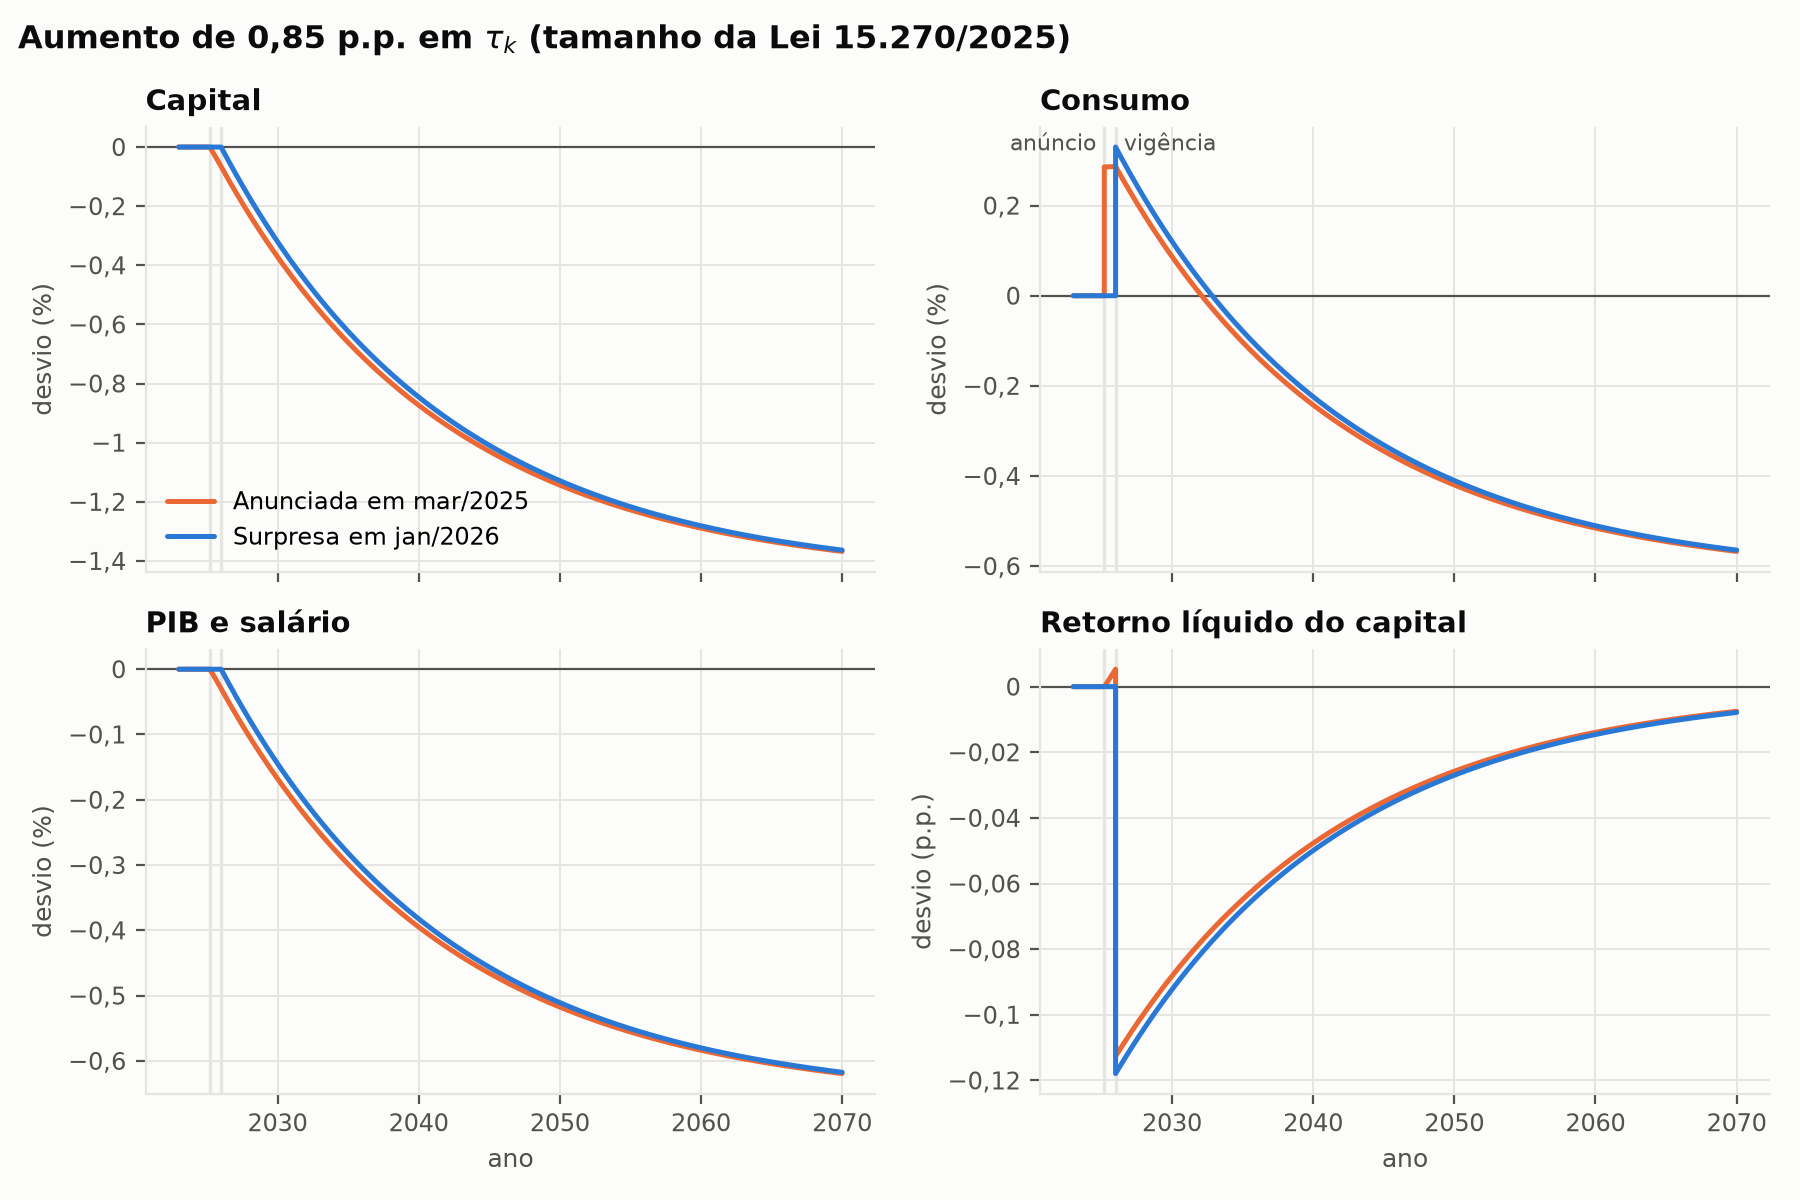
\includegraphics[width=\textwidth]{lei_15270.png}
\caption{Transição após o aumento de 0,85 p.p. em $\tau_k$: desvios em relação
à trajetória de crescimento balanceado inicial.}
\label{fig:lei}
\end{figure}

A Figura~\ref{fig:lei} mostra as trajetórias. Quando a notícia chega, o retorno
futuro da poupança cai e o consumo salta para cima: a família poupa menos.
O capital passa a cair e, com ele, o produto e os salários, até o novo estado
estacionário. No caso anunciado, o salto é um pouco menor e o capital já começa
a cair antes da vigência; o retorno líquido \emph{sobe} levemente nesse
intervalo, porque o capital fica mais escasso enquanto a alíquota antiga ainda
vale, e cai de uma vez na vigência. No longo prazo (Tabela~\ref{tab:sensibilidade},
linha ``base''), o capital cai 1,46\% e o PIB e os salários, 0,66\%. A
fórmula~\eqref{eq:elasticidade} dá o mesmo número à mão:
$-\frac{1}{0{,}549}\times\frac{0{,}138}{0{,}199}\times\frac{0{,}0085}{0{,}741}=-1{,}46\%$.

\paragraph{Receita estática e dinâmica.} Com o capital fixo, o aumento de
alíquota arrecadaria 0,268\% do PIB --- por construção, a estimativa oficial.
Depois que a base encolhe, a receita adicional de longo prazo é 0,242\% do PIB
inicial: 90\% da estimativa estática. A Figura~\ref{fig:laffer} mostra a curva
de Laffer de longo prazo do imposto sobre o capital: a receita máxima ocorre
em $\tau_k=66\%$, bem acima da alíquota atual, de modo que o Brasil está no
lado crescente da curva.

\paragraph{Bem-estar.} Com a receita devolvida como transferência, o aumento
de $\tau_k$ é pura distorção para a família representativa, e o custo é de
0,084\% do consumo em todas as datas, quase igual nos casos anunciado e
inesperado. Esse número não mede o objetivo distributivo da lei, que o modelo
não representa.

\begin{figure}[ht]
\centering
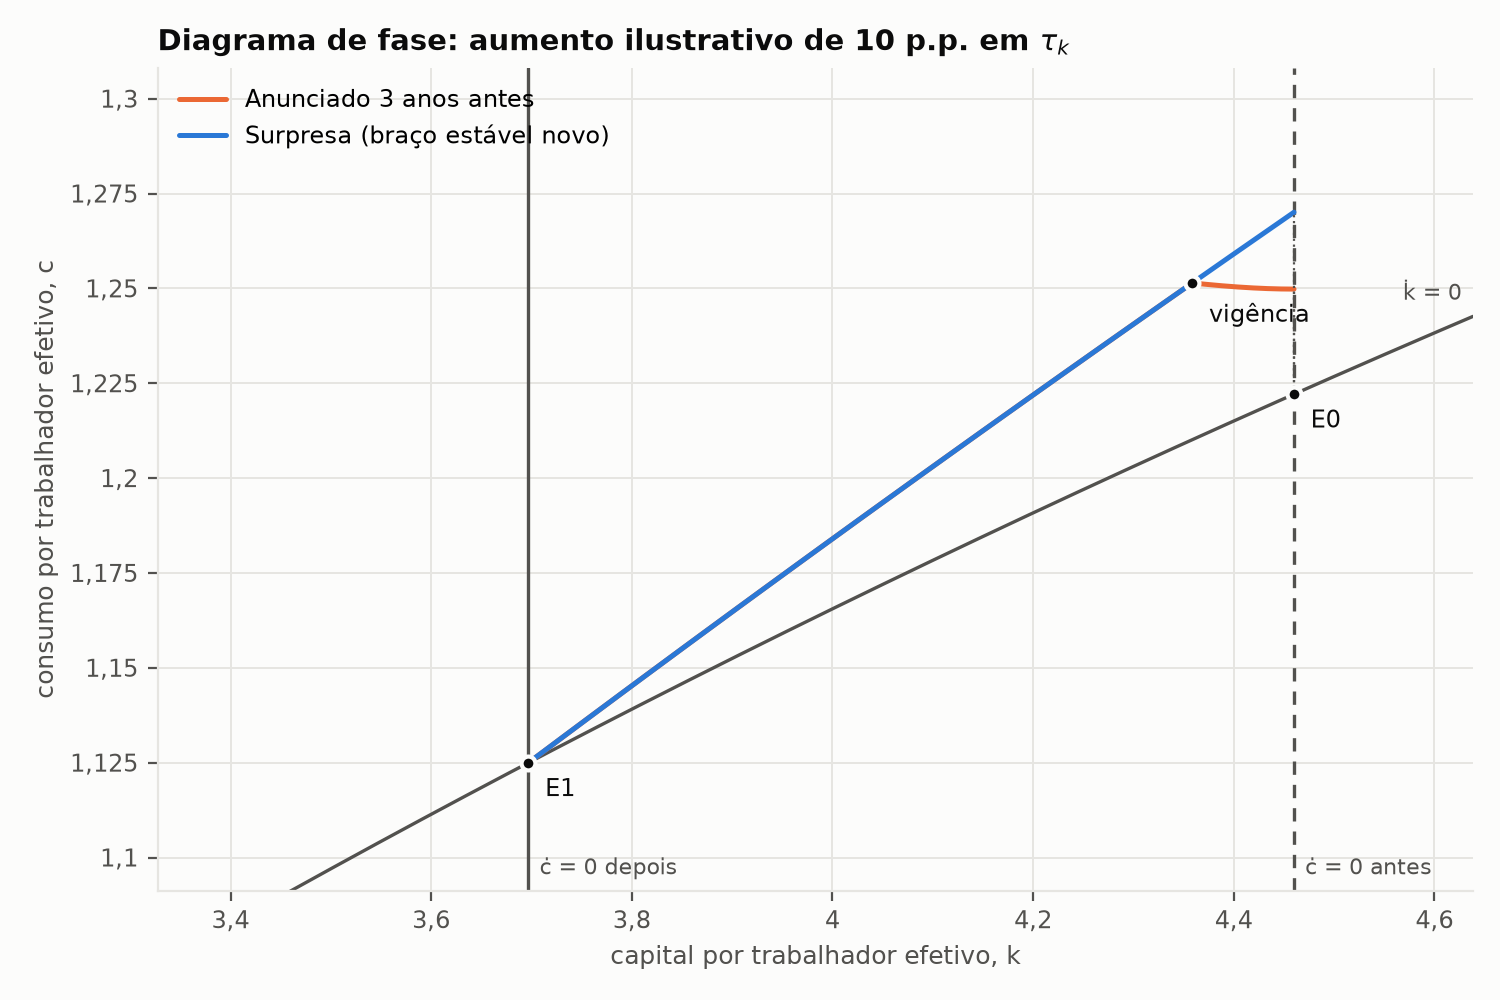
\includegraphics[width=0.82\textwidth]{diagrama_fase.png}
\caption{Diagrama de fase de um aumento ilustrativo de 10 p.p. em $\tau_k$.
A surpresa leva o consumo direto ao braço estável novo; o anúncio 3 anos antes
leva a uma trajetória instável sob a política antiga que alcança o braço estável
na vigência.}
\label{fig:fase}
\end{figure}

\begin{figure}[ht]
\centering
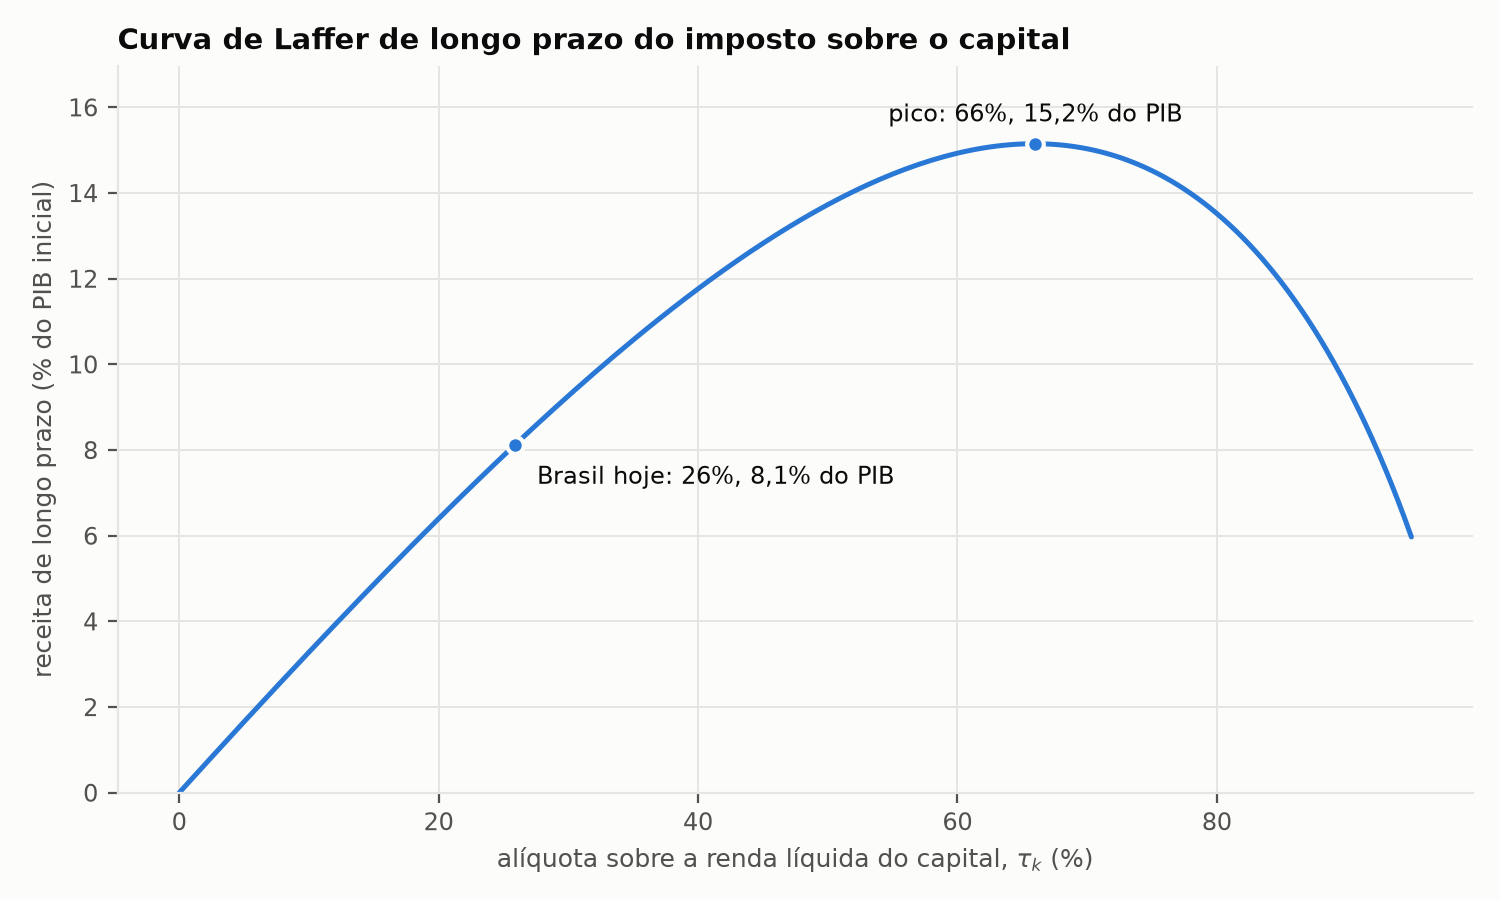
\includegraphics[width=0.82\textwidth]{laffer.png}
\caption{Receita de longo prazo do imposto sobre o capital, em \% do PIB
inicial. Como fração do próprio PIB ela é sempre crescente; a curva de Laffer
aparece em nível, porque $k^*\to0$ quando $\tau_k\to1$.}
\label{fig:laffer}
\end{figure}

\subsection{Sensibilidade}
Na Tabela~\ref{tab:sensibilidade}, $\rho$ é recalibrado em cada linha para
manter $K/Y$. Os efeitos de longo prazo não dependem de $\theta$: com $K/Y$
fixo, $r^*=\rho+\theta g$ é o mesmo e $k^*$ depende só dele e de $\tau_k$.
$\theta$ afeta apenas a transição e, por isso, o custo de bem-estar, que é maior
quando a substituição intertemporal é mais fácil ($\theta$ menor). Uma alíquota
inicial mais alta aumenta a perda de capital e de bem-estar e reduz a fração da
receita estática que sobrevive. Os efeitos crescem quase linearmente com o
tamanho do choque.

\begin{table}[ht]
\centering
\caption{Efeitos de longo prazo, receita e bem-estar (variações em \%)}
\label{tab:sensibilidade}
\small
\begin{tabular}{lccccccc}
\toprule
Caso & $\tau_k$ & Capital & PIB & Consumo & Receita & Receita & Bem-estar\\
 & inicial & & e salário & & estática & longo prazo & (surpresa)\\
\midrule
Base (+0,85 p.p.) & 0,259 & $-1{,}46$ & $-0{,}66$ & $-0{,}63$ & 0,268 & 0,242 & $-0{,}084$\\
$\theta=1$ & 0,259 & $-1{,}46$ & $-0{,}66$ & $-0{,}63$ & 0,268 & 0,242 & $-0{,}108$\\
$\theta=4$ & 0,259 & $-1{,}46$ & $-0{,}66$ & $-0{,}63$ & 0,268 & 0,242 & $-0{,}060$\\
$\tau_k^{\text{bruto}}=14\%$ & 0,201 & $-1{,}36$ & $-0{,}61$ & $-0{,}58$ & 0,268 & 0,249 & $-0{,}060$\\
$\tau_k^{\text{bruto}}=22\%$ & 0,316 & $-1{,}58$ & $-0{,}72$ & $-0{,}68$ & 0,268 & 0,233 & $-0{,}114$\\
Choque +2,5 p.p. & 0,259 & $-4{,}28$ & $-1{,}95$ & $-1{,}86$ & 0,784 & 0,701 & $-0{,}257$\\
Choque +5 p.p. & 0,259 & $-8{,}56$ & $-3{,}96$ & $-3{,}81$ & 1,569 & 1,381 & $-0{,}546$\\
\bottomrule
\end{tabular}

\smallskip
\footnotesize Receitas em \% do PIB inicial. Bem-estar em \% do consumo
(variação equivalente~\eqref{eq:lambda}).
\end{table}

\subsection{Outros choques}
A Figura~\ref{fig:outros} mostra dois experimentos que ilustram o papel das
expectativas. Um aumento de surpresa do gasto público de 2\% do PIB por cinco
anos, financiado por impostos lump-sum, derruba o consumo em cerca de 1,9\% de
imediato; como o choque é temporário, a família suaviza e absorve parte dele
reduzindo o investimento, e o capital cai 2,5\% até o fim do programa, com o
retorno subindo 0,2 p.p. Já um aumento de 5 p.p. no imposto sobre o consumo,
anunciado com dois anos de antecedência, antecipa consumo: o consumo sobe 1,7\%
no anúncio, cai na vigência exatamente pelo fator $(1{,}05)^{-1/2}$
de~\eqref{eq:salto} e volta ao nível inicial, pois $\tau_c$ constante é neutro no
longo prazo. A antecipação do consumo custa capital, que cai cerca de 1\% até a
vigência.

\begin{figure}[ht]
\centering
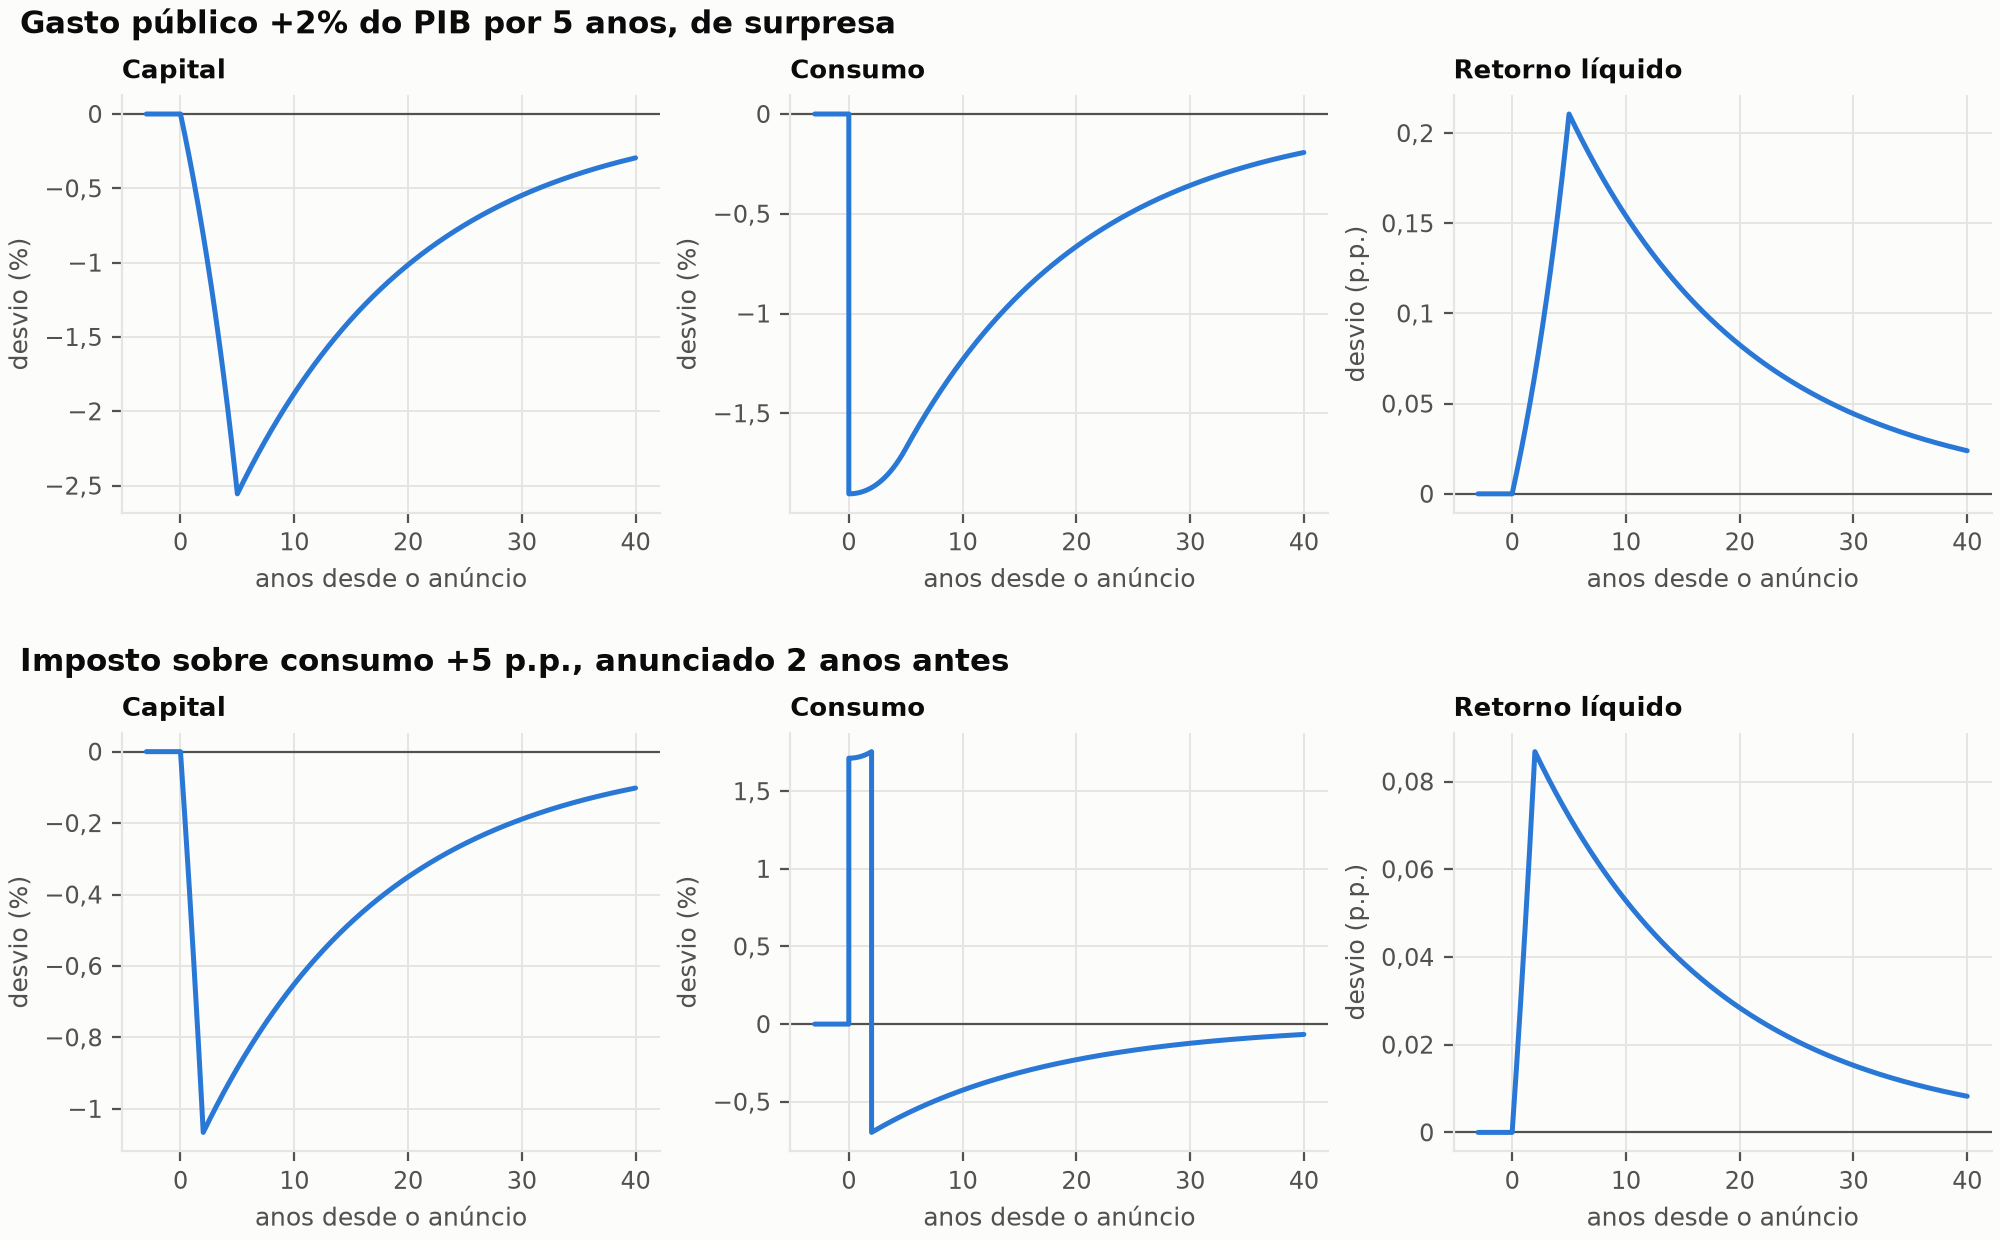
\includegraphics[width=\textwidth]{outros_choques.png}
\caption{Aumento temporário do gasto público e aumento anunciado do imposto
sobre o consumo.}
\label{fig:outros}
\end{figure}

\section{Estimação estrutural com dados sintéticos}
\label{sec:estimacao}

Calibrar $\rho$ a partir de $K/Y$ só identifica a combinação $r^*=\rho+\theta g$.
Esta seção pergunta se as \emph{transições} bastam para separar os dois
parâmetros, num experimento controlado em que o modelo é verdadeiro
(\texttt{estimacao.py}).

\paragraph{Equações de medida.} A economia calibrada parte de dois capitais
iniciais conhecidos, $0{,}6k^*$ e $1{,}4k^*$. Em cada ano $j=1,\dots,25$
observam-se o consumo agregado do ano e o capital no fim do ano,
\[
 \log C_j^{\text{obs}}=\log\int_{j-1}^{j}e^{(n+g)s}c(s)\dd s+\varepsilon_j^C,
 \qquad
 \log K_j^{\text{obs}}=\log\bigl[e^{(n+g)j}k(j)\bigr]+\varepsilon_j^K,
\]
com $\varepsilon^C,\varepsilon^K\sim N(0,\sigma^2)$ independentes e
$\sigma=0{,}01$. O consumo é um fluxo integrado no ano, e o capital, um estoque
numa data: misturá-los é um erro comum ao levar modelos contínuos aos dados.
As integrais usam quadratura de Gauss--Legendre com 16 nós.

\paragraph{Estimador.} Com os demais parâmetros fixos, $q=(\rho,\theta)$
minimiza a soma dos quadrados dos resíduos padronizados
$e_i(q)=[\log X_i^{\text{obs}}-\log X_i(q)]/\sigma$, resolvendo o equilíbrio a cada
avaliação. Sob o modelo correto, a covariância assintótica é
$(J'J)^{-1}$, com $J=\partial e/\partial q'$.

\paragraph{Resultados.} Numa amostra ($N=100$ observações), obtém-se
$\hat\rho=0{,}0893$ (0,0003) e $\hat\theta=1{,}933$ (0,025), com correlação de
$-0{,}72$ entre os estimadores. A Tabela~\ref{tab:mc} resume 100 réplicas: o
viés é desprezível, o erro-padrão médio coincide com a dispersão das
estimativas e os intervalos de 95\% cobrem o valor verdadeiro em 96\%--97\% das
réplicas. A Figura~\ref{fig:mc} mostra a identificação: as estimativas se
espalham ao longo da reta $\rho+\theta g=r^*$, que é o que o estado estacionário
identifica sozinho, e é a curvatura das transições que as prende em torno do
valor verdadeiro. Com dados reais, o exercício exigiria erros correlacionados,
parâmetros incertos e as extensões da Seção~\ref{sec:limites}; ele verifica o
algoritmo e a identificação, não a validade externa do modelo.

\begin{table}[ht]
\centering
\caption{Monte Carlo com 100 réplicas}
\label{tab:mc}
\begin{tabular}{lccccccc}
\toprule
 & Verdadeiro & Média & Viés & REQM & DP & EP médio & Cobertura 95\%\\
\midrule
$\rho$ & 0,0889 & 0,0890 & 0,0000 & 0,0003 & 0,0003 & 0,0003 & 0,97\\
$\theta$ & 2,000 & 1,995 & $-0{,}005$ & 0,027 & 0,027 & 0,026 & 0,96\\
\bottomrule
\end{tabular}
\end{table}

\begin{figure}[ht]
\centering
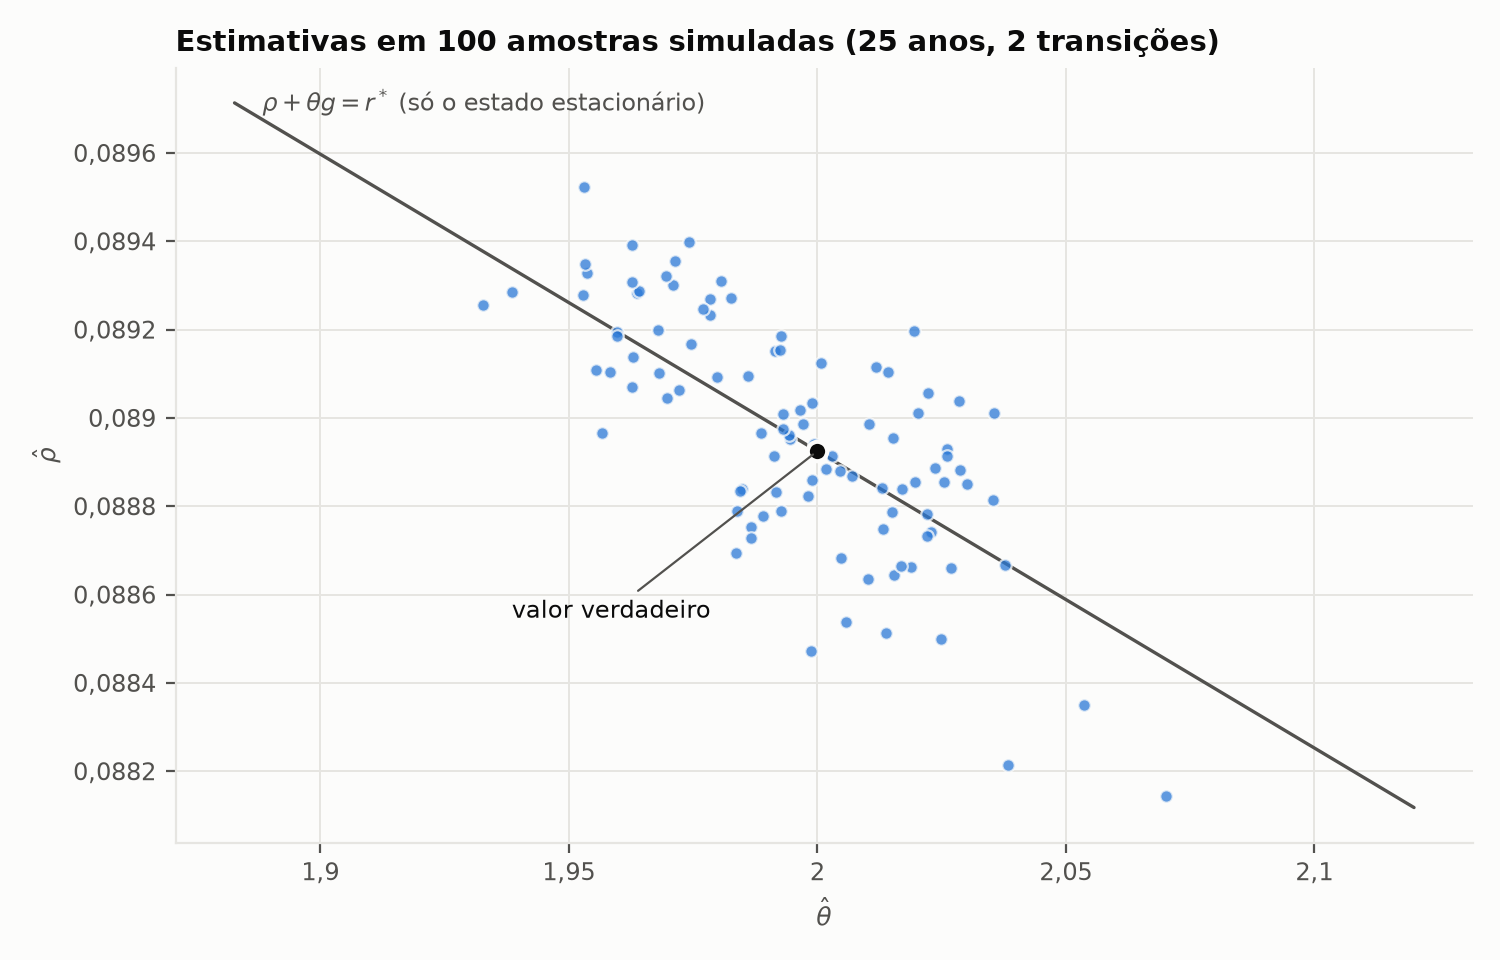
\includegraphics[width=0.78\textwidth]{monte_carlo.png}
\caption{Estimativas de $(\rho,\theta)$ nas 100 réplicas.}
\label{fig:mc}
\end{figure}

\section{Famílias heterogêneas}
\label{sec:ha}

O modelo representativo diz quanto a economia perde, mas não quem perde. Esta
seção substitui a família representativa por um contínuo de dinastias que
diferem em riqueza e renda e enfrentam risco de desemprego que não conseguem
segurar: o modelo de Aiyagari (1994), em tempo contínuo, como em Achdou et al.
(2022). Tecnologia, crescimento, gasto público e a alíquota $\tau_k$ são os da
Seção~\ref{sec:calibracao}.

\subsection{Modelo}
Cada dinastia tem riqueza por membro $a\ge0$, em unidades de eficiência, e
produtividade $z$, que segue uma cadeia de Markov em tempo contínuo com
intensidades $q_{zz'}$. Com $\tilde r=(1-\tau_k)r$ e $r=\alpha K^{\alpha-1}-\delta$,
\begin{equation}
 \dot a=(\tilde r-n-g)\,a+(1-\tau_w)\,w\,z+T_z-c,
 \label{eq:orcamento_ha}
\end{equation}
em que $\tau_w$ tributa a renda do trabalho e $T_z$ é uma transferência. A
função valor resolve a equação de Hamilton--Jacobi--Bellman
\begin{equation}
 \beta V_z(a)=\max_c\;u(c)+V_z'(a)\,\dot a+\sum_{z'}q_{zz'}\bigl[V_{z'}(a)-V_z(a)\bigr],
 \qquad \beta=\rho-n-(1-\theta)g,
 \label{eq:hjb}
\end{equation}
com $u'(c)=V_z'(a)$ e a restrição de estado $V_z'(0)\ge u'\bigl((1-\tau_w)wz+T_z\bigr)$,
que impede a riqueza de ficar negativa. A densidade estacionária $g_z(a)$
resolve a equação de Kolmogorov
\begin{equation}
 0=-\frac{\partial}{\partial a}\bigl[s_z(a)\,g_z(a)\bigr]+\sum_{z'}q_{z'z}\,g_{z'}(a)-\sum_{z'}q_{zz'}\,g_z(a),
 \label{eq:kfe}
\end{equation}
com $s_z(a)$ a poupança de~\eqref{eq:orcamento_ha}. O equilíbrio exige
$K=\sum_z\int a\,g_z(a)\dd a$, trabalho efetivo $E[z]=1$ e o orçamento do
governo $G+\bar T=\tau_k rK+\tau_w w$, com $\bar T$ a transferência média. O
seguro incompleto gera poupança precaucional, e por isso $\tilde r<\rho+\theta g$:
para sustentar o mesmo $K/Y$, as famílias precisam ser mais impacientes que no
modelo representativo. Sem risco, a regra de consumo é a do modelo representativo
(isso é um dos testes do código).

\subsection{Método numérico}
O código (\texttt{aiyagari.py}) segue Achdou et al. (2022). A equação HJB é
discretizada por diferenças finitas \emph{upwind} numa grade de riqueza mais
densa perto de zero, $a_i=150\,(i/599)^2$, e resolvida por iteração implícita.
A matriz $A$ das diferenças finitas é o gerador do processo $(a,z)$; sua
transposta discretiza~\eqref{eq:kfe}, o que garante que a distribuição conserve
massa. O equilíbrio estacionário é encontrado pelo método de Brent na taxa de
juros. Na calibração, $K/Y$ fixa $r$, e $\rho$ sai de um problema das famílias
por candidato.

A transição depois de uma mudança inesperada de política usa uma grade temporal
$t_n=150\,(n/200)^2$, com passos curtos no início: dado um caminho de $K(t)$,
resolve a HJB para trás a partir do novo estado estacionário, avança a
distribuição para frente a partir da antiga e atualiza $K(t)$ até a oferta de
capital igualar a demanda. Como a oferta de capital desse modelo reage muito aos
juros futuros, a atualização precisa ser amortecida: com peso de 0,3 no caminho
novo a iteração oscila e diverge; com 0,1 converge em cerca de 35 iterações.
Os testes conferem a regra de consumo exata sem risco, a restrição de recursos,
o orçamento do governo e a invariância dos resultados à grade.

\subsection{Calibração com a PNAD Contínua}
\paragraph{Risco de desemprego.} De 2012 a 2025, a desocupação média foi de 9,7\%,
e a distribuição do tempo de procura dos desocupados foi de 14,5\% com menos de
um mês, 49,4\% entre um mês e um ano, 14,4\% entre um e dois anos e 21,7\% com
dois anos ou mais (IBGE, tabelas 4099 e 1616). Se a saída do desemprego ocorre
a uma taxa constante $f$, o tempo já decorrido de procura de quem está
desempregado é exponencial com parâmetro $f$; uma única taxa, porém, não
reproduz ao mesmo tempo tantos episódios curtos e tantos longos. Com dois tipos
de desempregado, a distribuição é uma mistura de exponenciais, cujos três
parâmetros reproduzem exatamente as quatro faixas: 42\% dos desempregados são de
curta duração, com saída de 4,10 por ano (2,9 meses em média), e os demais saem
a 0,49 por ano (2 anos em média). A taxa de separação, 0,216 por ano, reproduz a
desocupação média; o episódio médio de desemprego dura 6 meses. Durante o
desemprego, a família recebe 40\% da sua renda do trabalho.

\paragraph{Desigualdade de renda.} Há três tipos permanentes, definidos pela
massa de rendimento do trabalho da PNAD (tabela 7543, média de 2012 a 2025): os
50\% com menor renda recebem 19,2\% da massa; os 40\% seguintes, 40,0\%; os
10\% com maior renda, 40,8\%. A produtividade relativa dos tipos é, portanto,
0,38, 1,00 e 4,10. O risco de desemprego é o mesmo para todos, o que é uma
simplificação.

\paragraph{Resultado.} Para reproduzir $K/Y=2{,}27$, a taxa de desconto é
$\rho=0{,}0903$, acima dos 0,0889 do modelo representativo, e $\tau_w=0{,}202$
financia o gasto que $\tau_k$ não cobre. O Gini da renda no modelo é 0,48,
perto do Gini do rendimento domiciliar per capita do IBGE (0,53 na média de
2012 a 2025). A riqueza, porém, é bem menos concentrada que nos dados: os 10\%
mais ricos têm 44\% da riqueza no modelo e cerca de 80\% no Brasil (World
Inequality Database, 2021), uma limitação conhecida desse tipo de modelo
(Castañeda, Díaz-Giménez e Ríos-Rull, 2003) ilustrada na Figura~\ref{fig:lorenz}.

\begin{figure}[ht]
\centering
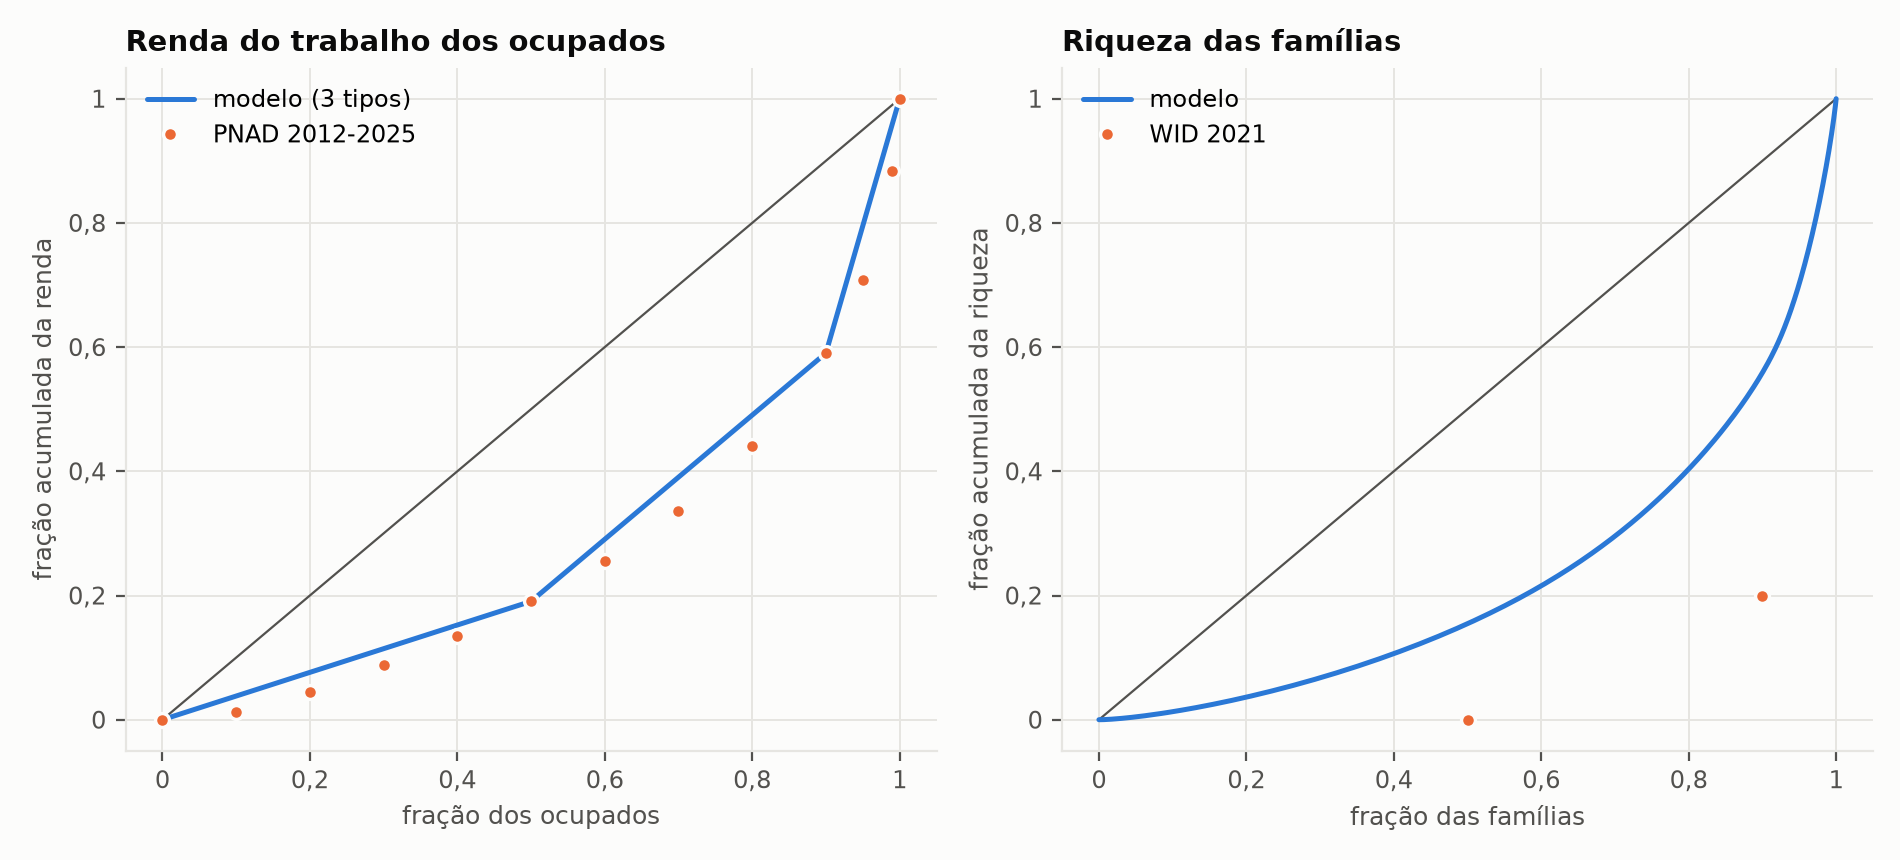
\includegraphics[width=\textwidth]{ha_lorenz.png}
\caption{Curvas de Lorenz do modelo e dos dados: renda do trabalho dos
ocupados (PNAD) e riqueza das famílias (WID).}
\label{fig:lorenz}
\end{figure}

\subsection{Quem ganha e quem perde}
O experimento é o da Seção~\ref{sec:calibracao}: $\tau_k$ aumenta 0,85 ponto
percentual de surpresa em $t=0$. A receita nova volta às famílias de duas
formas. Na devolução \emph{uniforme}, todas recebem a mesma transferência. Na
devolução \emph{isenção}, ela vai só para os empregados do grupo intermediário,
o que imita a isenção do imposto de renda da lei: pelos limites de percentil da
PNAD de 2025, o antigo limite de isenção (cerca de R\$ 3 mil) fica perto do P70
(R\$ 3.055), e o novo limite de R\$ 5 mil e a redução parcial até R\$ 7.350
ficam entre o P80 (R\$ 4.470) e o P90 (R\$ 6.985), todos dentro desse grupo.

O bem-estar de cada família $(a,z)$ é medido em $t=0$, incluindo toda a
transição: $\lambda(a,z)=[V^{\text{novo}}_0(a,z)/V^{\text{antigo}}(a,z)]^{1/(1-\theta)}-1$
é a fração do consumo, em todas as datas, que a deixaria indiferente entre a
reforma e o \emph{status quo}. A Tabela~\ref{tab:ha} resume os resultados, e as
Figuras~\ref{fig:grupos} e~\ref{fig:bemestar} os detalham.

\begin{table}[ht]
\centering
\caption{Efeitos do aumento de 0,85 p.p. em $\tau_k$ com famílias heterogêneas}
\label{tab:ha}
\begin{tabular}{lcccc}
\toprule
 & \multicolumn{2}{c}{Devolução uniforme} & \multicolumn{2}{c}{Devolução isenção}\\
\cmidrule(lr){2-3}\cmidrule(lr){4-5}
Grupo & Ganha (\%) & Ganho médio (\%) & Ganha (\%) & Ganho médio (\%)\\
\midrule
50\% com menor renda & 100 & $0{,}58$ & 0 & $-0{,}42$\\
40\% seguintes & 29 & $-0{,}06$ & 100 & $0{,}49$\\
10\% com maior renda & 0 & $-0{,}35$ & 0 & $-0{,}44$\\
Todos & 62 & $0{,}23$ & 40 & $-0{,}06$\\
\midrule
Capital de longo prazo & \multicolumn{2}{c}{$-1{,}45\%$} & \multicolumn{2}{c}{$-1{,}41\%$}\\
\bottomrule
\end{tabular}

\smallskip
\footnotesize Ganho: variação equivalente em \% do consumo, ponderada pela
distribuição inicial. No modelo representativo, todos perdem 0,084\% e o
capital cai 1,46\%.
\end{table}

\begin{figure}[ht]
\centering
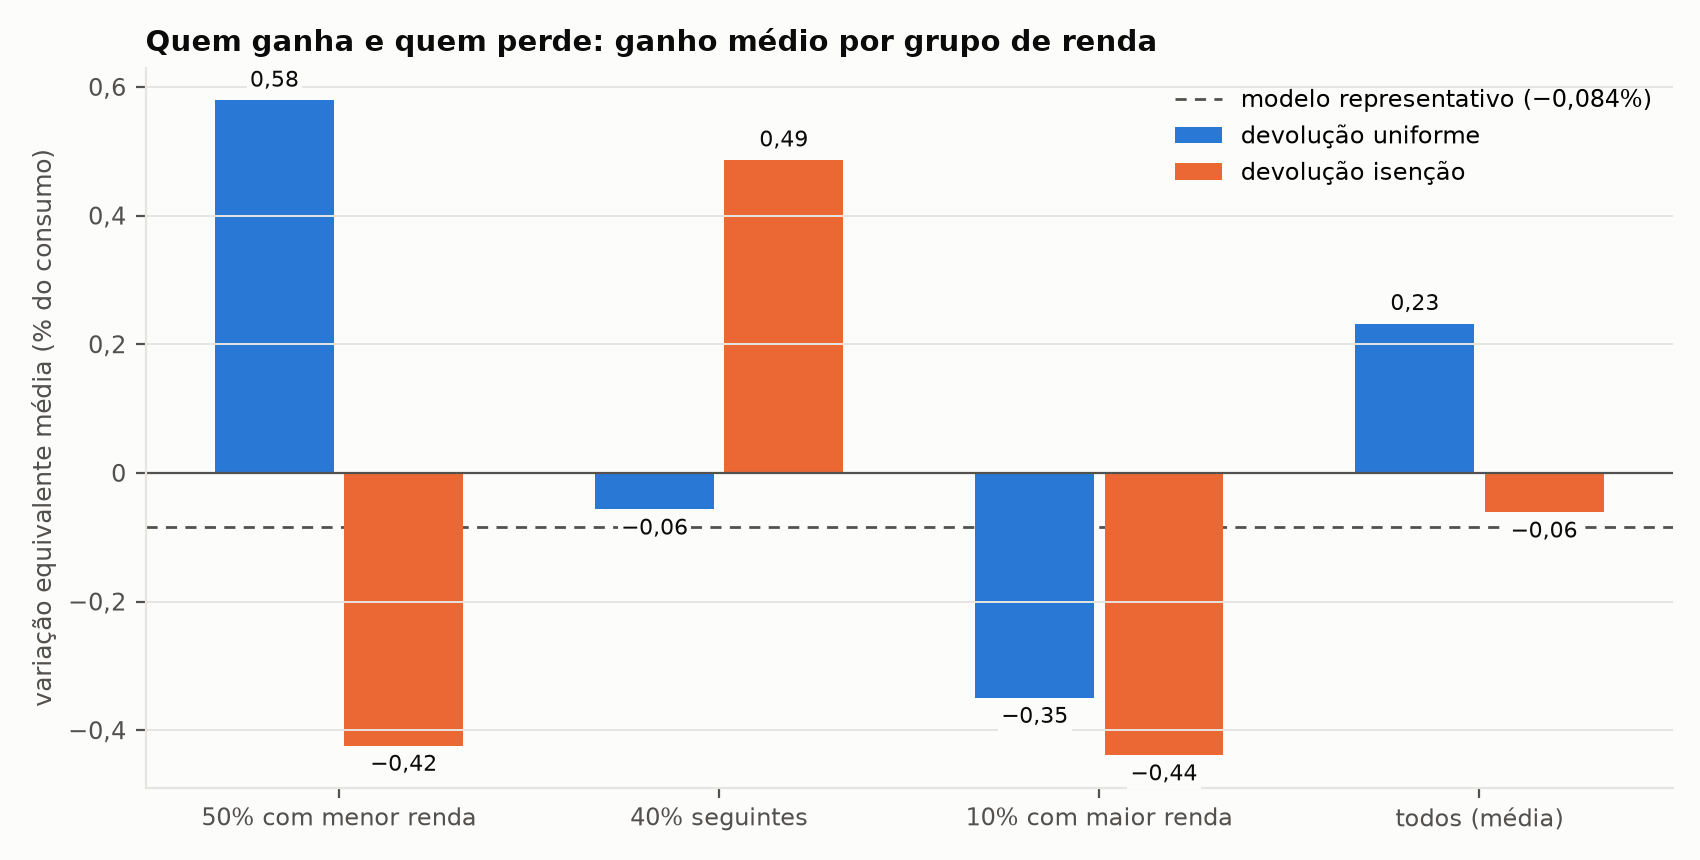
\includegraphics[width=0.85\textwidth]{ha_grupos.png}
\caption{Variação equivalente média por grupo de renda.}
\label{fig:grupos}
\end{figure}

\begin{figure}[ht]
\centering
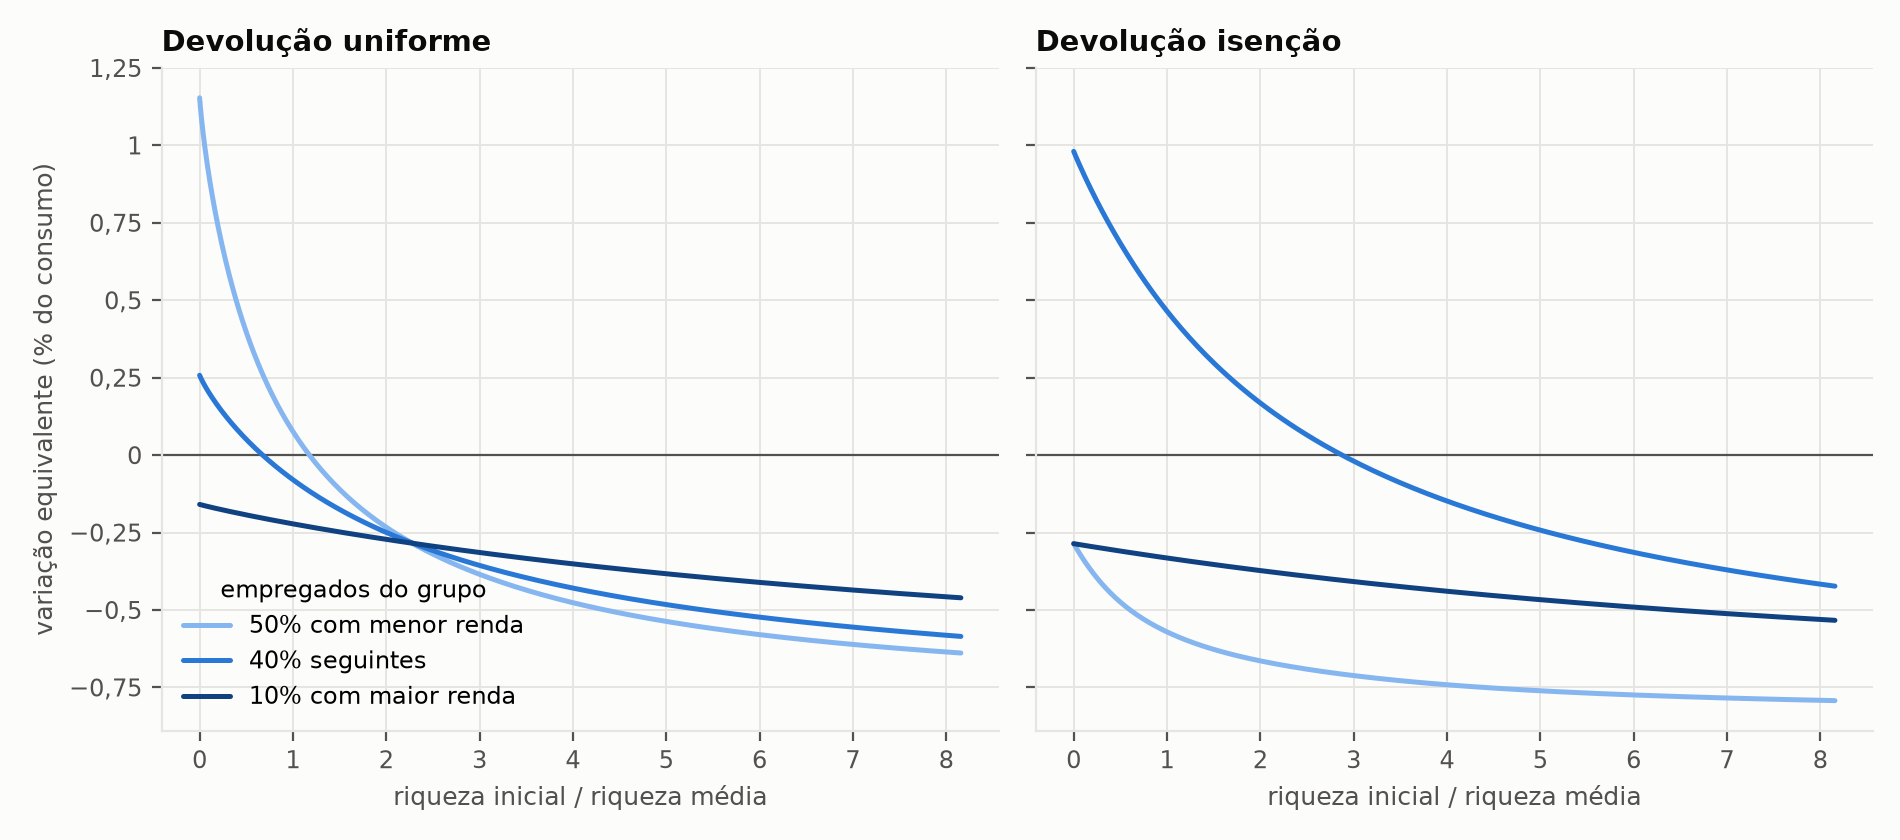
\includegraphics[width=\textwidth]{ha_bem_estar.png}
\caption{Variação equivalente dos empregados de cada grupo em função da riqueza
inicial.}
\label{fig:bemestar}
\end{figure}

Três resultados se destacam. \textbf{Primeiro}, o agregado é quase o mesmo do
modelo representativo: o capital de longo prazo cai 1,45\% ou 1,41\%, contra
1,46\%, e a transição tem velocidade parecida (Figura~\ref{fig:transicao_ha}).
Para medir o efeito sobre o PIB, o agente representativo é uma boa aproximação.

\textbf{Segundo}, a distribuição muda tudo. Com devolução uniforme, a
transferência vale muito mais, em proporção do consumo, para quem tem pouca
renda e pouca riqueza do que a queda gradual dos salários e dos juros: toda a
metade mais pobre ganha, e 62\% das famílias saem ganhando. O ganho cai com a
riqueza --- de $+0{,}82\%$ no décimo mais pobre a $-0{,}36\%$ no mais rico ---
porque os ricos pagam o imposto sobre o capital e vivem mais da renda do
capital, cujo retorno líquido cai.

\textbf{Terceiro}, com a devolução que imita a lei, os ganhadores são a faixa
intermediária, que recebe a isenção, e a metade mais pobre \emph{perde}
$0{,}42\%$: ela já era isenta e arca com a queda dos salários que a redução do
capital provoca. É o mesmo mecanismo que Domeij e Heathcote (2004) destacam
para a redução de impostos sobre o capital nos Estados Unidos, visto do outro
lado: os efeitos de equilíbrio geral sobre os salários distribuem o custo de
um imposto sobre o capital por toda a economia, inclusive por quem não o paga.

\begin{figure}[ht]
\centering
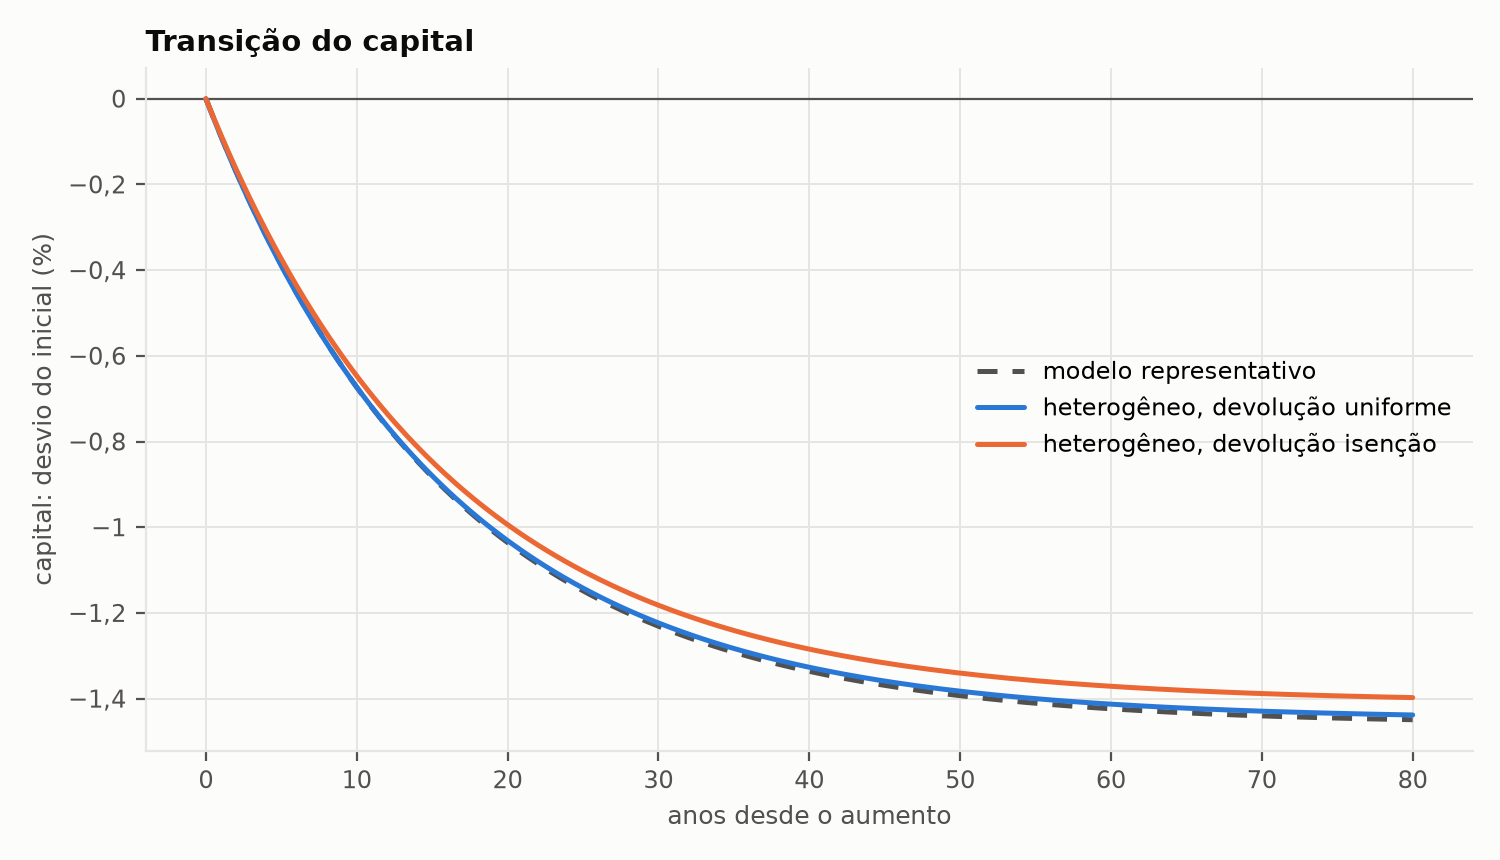
\includegraphics[width=0.8\textwidth]{ha_transicao.png}
\caption{Transição do capital no modelo representativo e no heterogêneo.}
\label{fig:transicao_ha}
\end{figure}

Esses números são condicionais às hipóteses do modelo: oferta de trabalho
inelástica, economia fechada, risco de desemprego igual para todos e riqueza
menos concentrada que nos dados. Com a concentração real, a perda dos mais ricos
e a receita seriam maiores. Além disso, a lei arrecada mais do que custa a
isenção (R\$ 34,12 bilhões contra R\$ 25,84 bilhões em 2026, nas estimativas
oficiais), e aqui toda a receita nova é devolvida.

\section{Limitações e extensões}
\label{sec:limites}

\begin{itemize}
 \item \textbf{Concentração da riqueza.} O modelo heterogêneo põe 44\% da
 riqueza nos 10\% mais ricos, contra cerca de 80\% nos dados. Retornos
 heterogêneos ou um estado de renda muito alta e raro (Castañeda et al., 2003)
 aproximariam o modelo dos dados.
 \item \textbf{Mercado de trabalho.} O risco de desemprego é o mesmo para todos
 os tipos e a informalidade não aparece; ambos pesam mais na base da
 distribuição.
 \item \textbf{Economia aberta.} Com mobilidade de capital, o retorno é
 ancorado no exterior e o imposto recai mais sobre o trabalho; a economia fechada
 é um caso extremo.
 \item \textbf{Oferta de trabalho.} Com trabalho elástico, a isenção para rendas
 baixas deixaria de ser neutra.
 \item \textbf{Incerteza.} O anúncio é tratado como crível; a tramitação do
 projeto foi incerta até a aprovação.
 \item \textbf{Medida da alíquota.} $\tau_k$ é uma alíquota média; decisões de
 investimento dependem da alíquota marginal efetiva, que pode ser diferente.
\end{itemize}

\section*{Reprodução}
Todos os números e figuras desta nota saem dos programas da pasta
\nolinkurl{Python/macroeconomia/equilibrio_geral}, a partir dos dados em
\nolinkurl{dados/brasil/}:
\begin{itemize}
 \item parte representativa: \texttt{calibracao.py}, \texttt{experimentos.py} e
 \texttt{estimacao.py -{}-replicas 100};
 \item famílias heterogêneas: \texttt{calibracao\_renda.py} e
 \texttt{experimentos\_ha.py}.
\end{itemize}

\begin{thebibliography}{99}
\small
\bibitem{achdou} Achdou, Y., Han, J., Lasry, J.-M., Lions, P.-L. e Moll, B. (2022).
Income and Wealth Distribution in Macroeconomics: A Continuous-Time Approach.
\emph{Review of Economic Studies}, 89(1), 45--86.
\bibitem{aiyagari} Aiyagari, S. R. (1994). Uninsured Idiosyncratic Risk and
Aggregate Saving. \emph{Quarterly Journal of Economics}, 109(3), 659--684.
\bibitem{acemoglu} Acemoglu, D. (2009). \emph{Introduction to Modern Economic
Growth}. Princeton University Press.
\bibitem{barro} Barro, R. J. e Sala-i-Martin, X. (2004). \emph{Economic Growth}.
2ª ed. MIT Press.
\bibitem{lei} Brasil (2025). Lei nº 15.270, de 26 de novembro de 2025.
\bibitem{em} Brasil, Ministério da Fazenda (2025). Exposição de Motivos
nº 00019/2025 MF, de 15 de março de 2025 (PL nº 1.087/2025).
\bibitem{castaneda} Castañeda, A., Díaz-Giménez, J. e Ríos-Rull, J.-V. (2003).
Accounting for the U.S. Earnings and Wealth Inequality. \emph{Journal of
Political Economy}, 111(4), 818--857.
\bibitem{cass} Cass, D. (1965). Optimum Growth in an Aggregative Model of Capital
Accumulation. \emph{Review of Economic Studies}, 32(3), 233--240.
\bibitem{chamley} Chamley, C. (1986). Optimal Taxation of Capital Income in
General Equilibrium with Infinite Lives. \emph{Econometrica}, 54(3), 607--622.
\bibitem{domeij} Domeij, D. e Heathcote, J. (2004). On the Distributional
Effects of Reducing Capital Taxes. \emph{International Economic Review}, 45(2),
523--554.
\bibitem{pwt} Feenstra, R. C., Inklaar, R. e Timmer, M. P. (2015). The Next
Generation of the Penn World Table. \emph{American Economic Review}, 105(10),
3150--3182. Dados: PWT 11.0 (2025).
\bibitem{gollin} Gollin, D. (2002). Getting Income Shares Right.
\emph{Journal of Political Economy}, 110(2), 458--474.
\bibitem{huggett} Huggett, M. (1993). The Risk-Free Rate in
Heterogeneous-Agent Incomplete-Insurance Economies. \emph{Journal of Economic
Dynamics and Control}, 17(5--6), 953--969.
\bibitem{ibge} IBGE. Pesquisa Nacional por Amostra de Domicílios Contínua.
SIDRA, tabelas 1616, 4099, 7435, 7536 e 7543.
\bibitem{judd85} Judd, K. L. (1985). Redistributive Taxation in a Simple
Perfect Foresight Model. \emph{Journal of Public Economics}, 28(1), 59--83.
\bibitem{judd98} Judd, K. L. (1998). \emph{Numerical Methods in Economics}.
MIT Press.
\bibitem{kierzenka} Kierzenka, J. e Shampine, L. F. (2001). A BVP Solver Based
on Residual Control and the MATLAB PSE. \emph{ACM Transactions on Mathematical
Software}, 27(3), 299--316.
\bibitem{koopmans} Koopmans, T. C. (1965). On the Concept of Optimal Economic
Growth. In \emph{The Econometric Approach to Development Planning}.
North-Holland.
\bibitem{mrt} Mendoza, E. G., Razin, A. e Tesar, L. L. (1994). Effective Tax
Rates in Macroeconomics: Cross-Country Estimates of Tax Rates on Factor Incomes
and Consumption. \emph{Journal of Monetary Economics}, 34(3), 297--323.
\bibitem{rabelo} Rabelo, T. C. (2025). Alíquotas Tributárias Médias Sobre o
Consumo e a Renda dos Fatores no Brasil 2000t1--2022t4. \emph{Cadernos de
Finanças Públicas}, 25(3).
\bibitem{ramsey} Ramsey, F. P. (1928). A Mathematical Theory of Saving.
\emph{Economic Journal}, 38(152), 543--559.
\bibitem{romer} Romer, D. (2019). \emph{Advanced Macroeconomics}. 5ª ed.
McGraw-Hill.
\bibitem{wid} World Inequality Database (2025). Brasil: distribuição da
riqueza líquida pessoal. Disponível em wid.world.
\end{thebibliography}

\end{document}
